\chapter{WebAIM: Screen Reader User Survey \#10 Results (2025)}
\glsreset{ocr}\glsreset{icr}\glsreset{tts}\glsreset{llm}\glsreset{uia}\glsreset{msaa}\glsreset{pdfua}\glsreset{api}\glsreset{cpu}
\label{cha:webaim-10}
\section{~~Introduction}
\label{sec:webaim-10-introduction}
This appendix contains the results of the 10th WebAIM Survey of Screen Reader\index{screen reader} Users, conducted in September, 2023\supercite{webaimsurvey10}. The survey was translated into 8 languages and promoted to various international mailing lists\index{Markdown!lists}. After filtering and removing invalid and duplicate responses, a total of 1539 valid responses were received.
\section{~~Demographics}
\label{sec:webaim-10-demographics}
This section presents demographic information about the survey respondents.
\subsection{Region}
\label{sec:webaim-10-region}
The following table shows the geographical distribution of respondents.
\begin{longtblr}[
		caption = {~~Region of Residence},
		label = {tab:webaim-10-region},
	]
	{
		colspec = {X[l] X[r] X[r]},
		rowhead = 1,
		row{1} = {font=\bfseries},
		hlines,
		stretch = 2
	}
	Region          & Number & Percent \\
	North America   & 630    & 41.0\%  \\
	Europe          & 528    & 34.3\%  \\
	Asia            & 189    & 12.3\%  \\
	South America   & 96     & 6.2\%   \\
	Africa          & 54     & 3.5\%   \\
	Oceania         & 33     & 2.1\%   \\
	Central America & 9      & 0.6\%   \\
\end{longtblr}
\subsection{Age}
\label{sec:webaim-10-age}
The following table shows the age distribution of respondents.
\begin{longtblr}[
		caption = {~~Age of Respondents},
		label = {tab:webaim-10-age},
	]
	{
		colspec = {X[l] X[r] X[r]},
		rowhead = 1,
		row{1} = {font=\bfseries},
		hlines,
		stretch = 2
	}
	Age   & Number & Percent \\
	18-20 & 63     & 4.1\%   \\
	21-40 & 681    & 44.3\%  \\
	41-60 & 591    & 38.4\%  \\
	61+   & 204    & 13.2\%  \\
\end{longtblr}
\subsection{Disability}
\label{sec:webaim-10-disability}
The following table shows the primary disability of respondents.
\begin{longtblr}[
		caption = {~~Primary Disability},
		label = {tab:webaim-10-disability},
	]
	{
		colspec = {X[l] X[r] X[r]},
		rowhead = 1,
		row{1} = {font=\bfseries},
		hlines,
		stretch = 2
	}
	Disability                   & Number & Percent \\
	Blindness                    & 1188   & 77.2\%  \\
	Low Vision/Visually Impaired & 243    & 15.8\%  \\
	Cognitive or Learning        & 48     & 3.1\%   \\
	Deaf or Hard-of-Hearing      & 30     & 1.9\%   \\
	Motor                        & 30     & 1.9\%   \\
\end{longtblr}
\subsection{Disability Types}
\label{sec:webaim-10-disability-types}
The following table shows the types of disabilities reported by respondents.
\begin{longtblr}[
		caption = {~~Disability Types},
		label = {tab:webaim-10-disability-types},
	]
	{
		colspec = {X[l] X[r] X[r]},
		rowhead = 1,
		row{1} = {font=\bfseries},
		hlines,
		stretch = 2
	}
	Disability Type              & Number & Percent \\
	Blindness                    & 1206   & 78.4\%  \\
	Low Vision/Visually Impaired & 303    & 19.7\%  \\
	Cognitive or Learning        & 129    & 8.4\%   \\
	Motor                        & 93     & 6.0\%   \\
	Deaf or Hard-of-Hearing      & 87     & 5.7\%   \\
	Other                        & 114    & 7.4\%   \\
\end{longtblr}
\subsection{Screen Reader Proficiency}
\label{sec:webaim-10-screen-reader-proficiency}
The following table shows the self-reported screen reader proficiency\index{screen reader!screen reader proficiency} of respondents.
\begin{longtblr}[
		caption = {~~Screen Reader Proficiency},
		label = {tab:webaim-10-screen-reader-proficiency},
	]
	{
		colspec = {X[l] X[r] X[r]},
		rowhead = 1,
		row{1} = {font=\bfseries},
		hlines,
		stretch = 2
	}
	Proficiency  & Number & Percent \\
	Advanced     & 843    & 54.8\%  \\
	Intermediate & 591    & 38.4\%  \\
	Beginner     & 105    & 6.8\%   \\
\end{longtblr}
\subsection{Internet Proficiency}
\label{sec:webaim-10-internet-proficiency}
The following table shows the self-reported internet proficiency of respondents.
\begin{longtblr}[
		caption = {~~Internet Proficiency},
		label = {tab:webaim-10-internet-proficiency},
	]
	{
		colspec = {X[l] X[r] X[r]},
		rowhead = 1,
		row{1} = {font=\bfseries},
		hlines,
		stretch = 2
	}
	Proficiency  & Number & Percent \\
	Advanced     & 1029   & 66.9\%  \\
	Intermediate & 468    & 30.4\%  \\
	Beginner     & 42     & 2.7\%   \\
\end{longtblr}

\section{~~Primary Desktop/Laptop Screen Reader}
\begin{figure}[htbp]
	\centering
	\imgalt{Historical trends in primary desktop/laptop screen reader usage (JAWS, NVDA, VoiceOver, Narrator).}{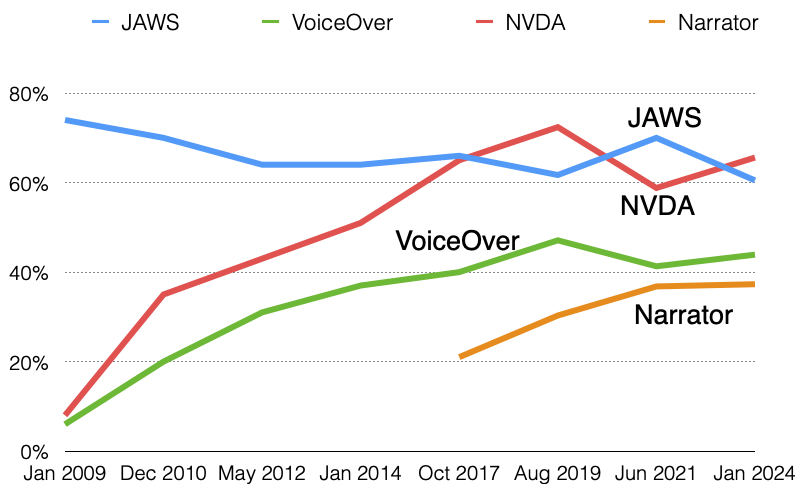
\includegraphics[width=0.8\linewidth]{SR-2.png}}
	\caption{Historical trends in primary desktop/laptop screen reader usage.}
	\label{fig:primary-desktop-laptop-screen-reader}
\end{figure}
\label{sec:webaim-10-primary-desktop-laptop-screen-reader}
The following table shows the primary desktop/laptop \gidx{screenreader}{screen reader} used by respondents.
\begin{longtblr}[
		caption = {~~Primary Desktop/Laptop Screen Reader},
		label = {tab:webaim-10-primary-desktop-laptop-screen-reader},
	]
	{
		colspec = {X[l] X[r] X[r]},
		rowhead = 1,
		row{1} = {font=\bfseries},
		hlines,
		stretch = 2
	}
	Screen Reader\index{screen reader}     & Number & Percent \\
	JAWS\index{screen reader!JAWS}         & 747    & 48.5\%  \\
	\gls{nvda}                             & 537    & 34.9\%  \\
	VoiceOver                              & 156    & 10.1\%  \\
	Narrator\index{screen reader!Narrator} & 39     & 2.5\%   \\
	Other                                  & 51     & 3.3\%   \\
\end{longtblr}
\section{~~Screen Readers Commonly Used}
\label{sec:webaim-10-screen-readers-commonly-used}
\begin{figure}[htbp]
	\centering
	\imgalt{Historical trends in overall screen reader usage (JAWS, NVDA, VoiceOver, Narrator) from 2009 to 2024.}{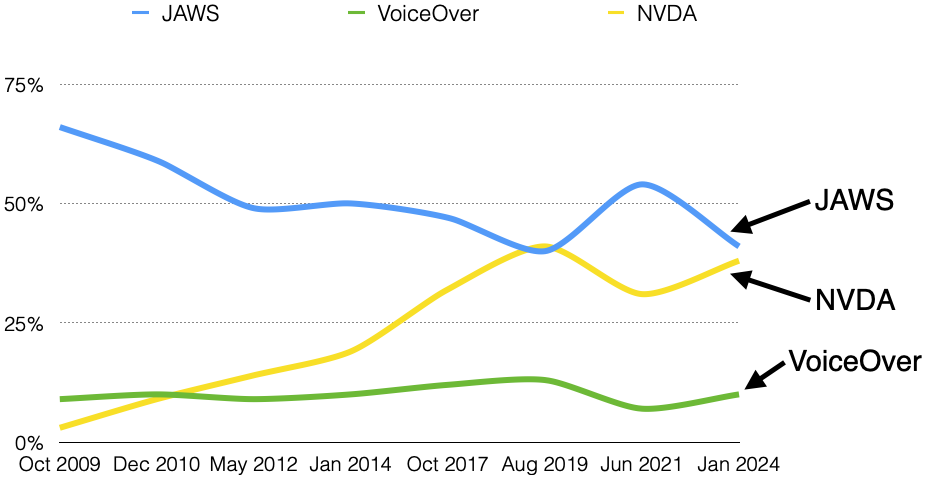
\includegraphics[width=0.8\linewidth]{SR-1}}
	\caption{Historical trends in commonly used screen readers.}
	\label{fig:screen-readers-commonly-used}
\end{figure}The following table shows the \gls{screenreader} commonly used by respondents.
\begin{longtblr}[
		caption = {~~Screen Readers Commonly Used},
		label = {tab:webaim-10-screen-readers-commonly-used},
	]
	{
		colspec = {X[l] X[r] X[r]},
		rowhead = 1,
		row{1} = {font=\bfseries},
		hlines,
		stretch = 2
	}
	Screen Reader                            & Number & Percent \\
	\gls{jaws}                               & 1029   & 66.9\%  \\
	NVDA                                     & 903    & 58.7\%  \\
	VoiceOver\index{screen reader!VoiceOver} & 489    & 31.8\%  \\
	\gls{narrator}                           & 381    & 24.8\%  \\
	Other                                    & 129    & 8.4\%   \\
\end{longtblr}
\section{~~Browsers}
\label{sec:webaim-10-browsers}
The following table shows the browsers used by respondents.
\begin{longtblr}[
		caption = {~~Browsers},
		label = {tab:webaim-10-browsers},
	]
	{
		colspec = {X[l] X[r] X[r]},
		rowhead = 1,
		row{1} = {font=\bfseries},
		hlines,
		stretch = 2
	}
	Browser & Number & Percent \\
	Chrome  & 789    & 51.3\%  \\
	Edge    & 381    & 24.8\%  \\
	Firefox & 267    & 17.4\%  \\
	Safari  & 63     & 4.1\%   \\
	Other   & 30     & 1.9\%   \\
\end{longtblr}
\imgalt{Historical trends in browser usage showing increase in Edge and Chrome over time and drop of Internet Explorer. Firefox, and Safari.}{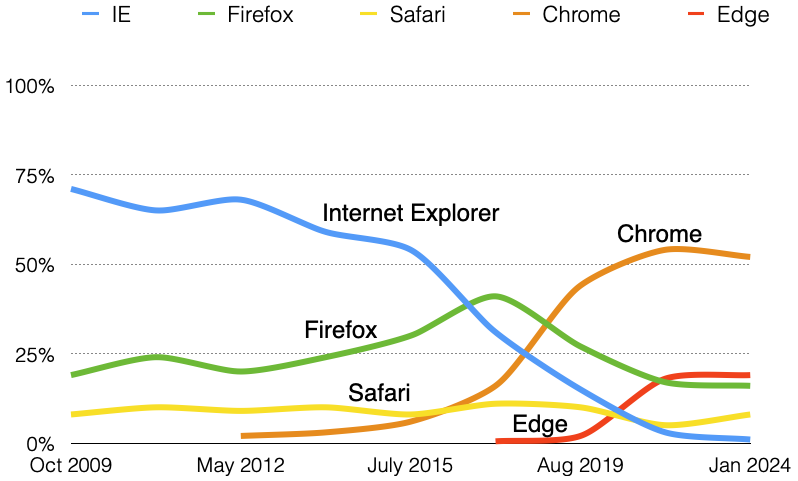
\includegraphics[width=0.8\linewidth]{browsers}}

\section{~~Screen Reader / Browser Combinations}
\label{sec:webaim-10-screen-reader-browser-combinations}
The following table shows the screen reader and browser combinations used by respondents.
\begin{longtblr}[
		caption = {~~Screen Reader / Browser Combinations},
		label = {tab:webaim-10-screen-reader-browser-combinations},
	]
	{
		colspec = {X[l] X[r] X[r]},
		rowhead = 1,
		row{1} = {font=\bfseries},
		hlines,
		stretch = 2
	}
	Combination                                 & Number & Percent \\
	JAWS with Chrome                            & 489    & 31.8\%  \\
	JAWS with Edge                              & 243    & 15.8\%  \\
	NVDA with Chrome                            & 225    & 14.6\%  \\
	NVDA\index{accessibility!NVDA} with Firefox & 189    & 12.3\%  \\
	VoiceOver with Safari                       & 129    & 8.4\%   \\
	Other                                       & 264    & 17.2\%  \\
\end{longtblr}
\section{~~Operating System}
\label{sec:webaim-10-operating-system}
The following table shows the operating systems used by respondents.
\begin{longtblr}[
		caption = {~~Operating System},
		label = {tab:webaim-10-operating-system},
	]
	{
		colspec = {X[l] X[r] X[r]},
		rowhead = 1,
		row{1} = {font=\bfseries},
		hlines,
		stretch = 2
	}
	\gls{operatingsystem}                     & Number & Percent \\
	Windows\index{operating system!Windows}   & 1329   & 86.4\%  \\
	macOS                                     & 156    & 10.1\%  \\
	Linux                                     & 33     & 2.1\%   \\
	ChromeOS\index{operating system!ChromeOS} & 12     & 0.8\%   \\
	Other                                     & 9      & 0.6\%   \\
\end{longtblr}
\section{~~JavaScript}
\label{sec:webaim-10-javascript}
The following table shows the percentage of respondents who have JavaScript enabled.
\begin{longtblr}[
		caption = {~~JavaScript Enabled},
		label = {tab:webaim-10-javascript-enabled},
	]
	{
		colspec = {X[l] X[r] X[r]},
		rowhead = 1,
		row{1} = {font=\bfseries},
		hlines,
		stretch = 2
	}
	Response & Number & Percent \\
	Yes      & 1509   & 98.1\%  \\
	No       & 30     & 1.9\%   \\
\end{longtblr}
\section{~~Reason for Use}
\label{sec:webaim-10-reason-for-use}
The following table shows the primary reason respondents use a \gidx{screenreader}{screen reader}.
\begin{longtblr}[
		caption = {~~Reason for Use},
		label = {tab:webaim-10-reason-for-use},
	]
	{
		colspec = {X[l] X[r] X[r]},
		rowhead = 1,
		row{1} = {font=\bfseries},
		hlines,
		stretch = 2
	}
	Reason                                                           & Number & Percent \\
	Disability                                                       & 1419   & 92.2\%  \\
	Accessibility Testing\index{accessibility!accessibility testing} & 90     & 5.8\%   \\
	Other                                                            & 30     & 1.9\%   \\
\end{longtblr}
\section{~~Screen Reader Satisfaction}
\label{sec:webaim-10-screen-reader-satisfaction}
The following table shows the satisfaction level of respondents with their primary screen reader\index{screen reader!primary screen reader}.
\begin{longtblr}[
		caption = {~~Screen Reader Satisfaction},
		label = {tab:webaim-10-screen-reader-satisfaction},
	]
	{
		colspec = {X[l] X[r] X[r]},
		rowhead = 1,
		row{1} = {font=\bfseries},
		hlines,
		stretch = 2
	}
	Satisfaction       & Number & Percent \\
	Very Satisfied     & 789    & 51.3\%  \\
	Satisfied          & 603    & 39.2\%  \\
	Somewhat Satisfied & 117    & 7.6\%   \\
	Dissatisfied       & 21     & 1.4\%   \\
	Very Dissatisfied  & 9      & 0.6\%   \\
\end{longtblr}
\section{~~Home vs. Work}
\label{sec:webaim-10-home-vs-work}
The following table shows where respondents primarily use their screen reader.
\begin{longtblr}[
		caption = {~~Home vs. Work},
		label = {tab:webaim-10-home-vs-work},
	]
	{
		colspec = {X[l] X[r] X[r]},
		rowhead = 1,
		row{1} = {font=\bfseries},
		hlines,
		stretch = 2
	}
	Location & Number & Percent \\
	Home     & 981    & 63.7\%  \\
	Work     & 351    & 22.8\%  \\
	Both     & 207    & 13.5\%  \\
\end{longtblr}
\section{~~Braille Output}
\label{sec:webaim-10-braille-output}
The following table shows the percentage of respondents who use a \gidx{brailledisplay}{braille display}.
\begin{longtblr}[
		caption = {~~Braille Output},
		label = {tab:webaim-10-braille-output},
	]
	{
		colspec = {X[l] X[r] X[r]},
		rowhead = 1,
		row{1} = {font=\bfseries},
		hlines,
		stretch = 2
	}
	Response & Number & Percent \\
	Yes      & 489    & 31.8\%  \\
	No       & 1050   & 68.2\%  \\
\end{longtblr}
\section{~~Free/Low-cost vs. Commercial}
\label{sec:webaim-10-free-low-cost-vs-commercial}
The following table shows the preference for free/low-cost vs. commercial screen readers\index{screen reader}.
\begin{longtblr}[
		caption = {~~Free/Low-cost vs. Commercial},
		label = {tab:webaim-10-free-low-cost-vs-commercial},
	]
	{
		colspec = {X[l] X[r] X[r]},
		rowhead = 1,
		row{1} = {font=\bfseries},
		hlines,
		stretch = 2
	}
	Preference    & Number & Percent \\
	Free/Low-cost & 843    & 54.8\%  \\
	Commercial    & 489    & 31.8\%  \\
	No Preference & 207    & 13.5\%  \\
\end{longtblr}
\section{~~Mobile Screen Readers}
\label{sec:webaim-10-mobile-screen-readers}
This section presents information about mobile screen reader usage.
\subsection{Mobile Usage}
\label{sec:webaim-10-mobile-usage}
The following table shows the percentage of respondents who use a screen reader on a mobile device.
\begin{longtblr}[
		caption = {~~Mobile Usage},
		label = {tab:webaim-10-mobile-usage},
	]
	{
		colspec = {X[l] X[r] X[r]},
		rowhead = 1,
		row{1} = {font=\bfseries},
		hlines,
		stretch = 2
	}
	Response & Number & Percent \\
	Yes      & 1329   & 86.4\%  \\
	No       & 210    & 13.6\%  \\
\end{longtblr}
\subsection{Mobile Platforms}
\begin{figure}[htbp]
	\centering
	\imgalt{Historical mobile platform usage showing iOS dominance and Android growth over time.}{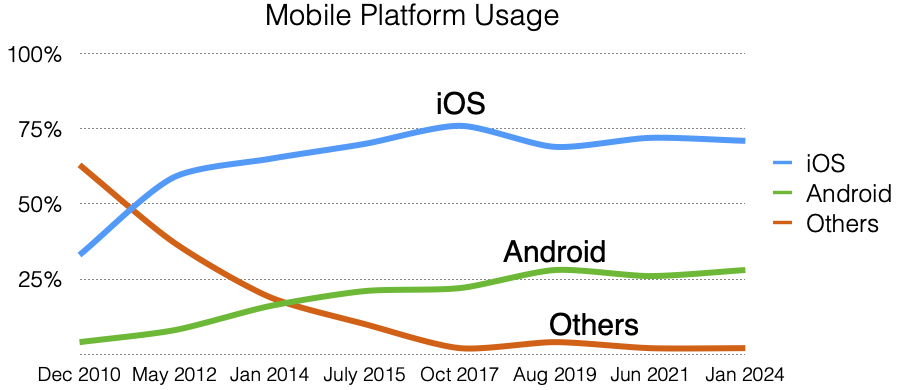
\includegraphics[width=0.8\linewidth]{mobile2}}
	\caption{Trends in mobile platform usage among screen reader users.}
	\label{fig:mobile-platform-trends}
\end{figure}
\label{sec:webaim-10-mobile-platforms}
The following table shows the mobile platforms used by respondents.
\begin{longtblr}[
		caption = {~~Mobile Platforms},
		label = {tab:webaim-10-mobile-platforms},
	]
	{
		colspec = {X[l] X[r] X[r]},
		rowhead = 1,
		row{1} = {font=\bfseries},
		hlines,
		stretch = 2
	}
	Platform                                & Number & Percent \\
	iOS                                     & 981    & 63.7\%  \\
	Android\index{operating system!Android} & 330    & 21.4\%  \\
	Other                                   & 18     & 1.2\%   \\
\end{longtblr}
\subsection{Mobile Screen Readers Used}
\label{sec:webaim-10-mobile-screen-readers-used}
The following table shows the mobile screen readers\index{screen reader!primary screen reader} used by respondents.
\begin{longtblr}[
		caption = {~~Mobile Screen Readers Used},
		label = {tab:webaim-10-mobile-screen-readers-used},
	]
	{
		colspec = {X[l] X[r] X[r]},
		rowhead = 1,
		row{1} = {font=\bfseries},
		hlines,
		stretch = 2
	}
	Screen Reader                            & Number & Percent \\
	VoiceOver\index{screen reader!VoiceOver} & 981    & 63.7\%  \\
	TalkBack\index{screen reader!TalkBack}   & 330    & 21.4\%  \\
	Other                                    & 18     & 1.2\%   \\
\end{longtblr}
\subsection{Primary Mobile Browser}
\label{sec:webaim-10-primary-mobile-browser}
The following table shows the primary mobile browser used by respondents.
\begin{longtblr}[
		caption = {~~Primary Mobile Browser},
		label = {tab:webaim-10-primary-mobile-browser},
	]
	{
		colspec = {X[l] X[r] X[r]},
		rowhead = 1,
		row{1} = {font=\bfseries},
		hlines,
		stretch = 2
	}
	Browser & Number & Percent \\
	Safari  & 981    & 63.7\%  \\
	Chrome  & 330    & 21.4\%  \\
	Firefox & 18     & 1.2\%   \\
	Other   & 9      & 0.6\%   \\
\end{longtblr}
\subsection{Mobile vs. Desktop/Laptop Usage}
\label{sec:webaim-10-mobile-vs-desktop-laptop-usage}
The following table shows the comparison of mobile vs. desktop/laptop\index{laptop} usage.
\begin{longtblr}[
		caption = {~~Mobile vs. Desktop/Laptop Usage},
		label = {tab:webaim-10-mobile-vs-desktop-laptop-usage},
	]
	{
		colspec = {X[l] X[r] X[r]},
		rowhead = 1,
		row{1} = {font=\bfseries},
		hlines,
		stretch = 2
	}
	Usage                             & Number & Percent \\
	More Desktop/Laptop\index{laptop} & 789    & 51.3\%  \\
	More Mobile                       & 489    & 31.8\%  \\
	About the Same                    & 261    & 17.0\%  \\
\end{longtblr}
\subsection{Mobile App vs Web Site Usage}
\label{sec:webaim-10-mobile-app-vs-web-site-usage}
The following table shows the preference for mobile apps\index{apps} vs. web sites.
\begin{longtblr}[
		caption = {~~Mobile App vs Web Site Usage},
		label = {tab:webaim-10-mobile-app-vs-web-site-usage},
	]
	{
		colspec = {X[l] X[r] X[r]},
		rowhead = 1,
		row{1} = {font=\bfseries},
		hlines,
		stretch = 2
	}
	Preference             & Number & Percent \\
	Mobile App\index{apps} & 843    & 54.8\%  \\
	Web Site               & 489    & 31.8\%  \\
	No Preference          & 207    & 13.5\%  \\
\end{longtblr}
\section{~~Web Accessibility Progress}
\label{sec:webaim-10-web-accessibility-progress}
The following table shows the perception of web accessibility progress\index{web accessibility!web accessibility progress} over the last year.
\begin{longtblr}[
		caption = {~~Web Accessibility Progress},
		label = {tab:webaim-10-web-accessibility-progress},
	]
	{
		colspec = {X[l] X[r] X[r]},
		rowhead = 1,
		row{1} = {font=\bfseries},
		hlines,
		stretch = 2
	}
	Perception      & Number & Percent \\
	More Accessible & 789    & 51.3\%  \\
	Less Accessible & 243    & 15.8\%  \\
	About the Same  & 507    & 33.0\%  \\
\end{longtblr}
\section{~~Impacts on Accessibility}
\label{sec:webaim-10-impacts-on-accessibility}
The following table shows the items that have the most impact on \gidx{accessibility}{accessibility}.
\begin{longtblr}[
		caption = {~~Impacts on Accessibility},
		label = {tab:webaim-10-impacts-on-accessibility},
	]
	{
		colspec = {X[l] X[r] X[r]},
		rowhead = 1,
		row{1} = {font=\bfseries},
		hlines,
		stretch = 2
	}
	Item                                                          & Number & Percent \\
	Properly Labeled Forms                                        & 1029   & 66.9\%  \\
	Proper Heading Structure                                      & 903    & 58.7\%  \\
	Images with Alt Text\index{images and media!alternative text} & 843    & 54.8\%  \\
	Keyboard \gls{accessibility}                                  & 789    & 51.3\%  \\
	ARIA Landmarks\index{web accessibility!landmarks}             & 681    & 44.3\%  \\
\end{longtblr}
\section{~~Descriptions in Virtual Meetings}
\label{sec:webaim-10-descriptions-in-virtual-meetings}
The following table shows the importance of descriptions in virtual meetings.
\begin{longtblr}[
		caption = {~~Descriptions in Virtual Meetings},
		label = {tab:webaim-10-descriptions-in-virtual-meetings},
	]
	{
		colspec = {X[l] X[r] X[r]},
		rowhead = 1,
		row{1} = {font=\bfseries},
		hlines,
		stretch = 2
	}
	Importance         & Number & Percent \\
	Very Important     & 981    & 63.7\%  \\
	Important          & 489    & 31.8\%  \\
	Somewhat Important & 60     & 3.9\%   \\
	Not Important      & 9      & 0.6\%   \\
\end{longtblr}
\section{~~Landmarks/Regions}
\label{sec:webaim-10-landmarks-regions}
The following table shows how often respondents use landmarks/regions to navigate web pages.
\begin{longtblr}[
		caption = {~~Landmarks/Regions},
		label = {tab:webaim-10-landmarks-regions},
	]
	{
		colspec = {X[l] X[r] X[r]},
		rowhead = 1,
		row{1} = {font=\bfseries},
		hlines,
		stretch = 2
	}
	Frequency & Number & Percent \\
	Always    & 489    & 31.8\%  \\
	Often     & 603    & 39.2\%  \\
	Sometimes & 330    & 21.4\%  \\
	Rarely    & 96     & 6.2\%   \\
	Never     & 21     & 1.4\%   \\
\end{longtblr}
\section{~~Finding Information}
\label{sec:webaim-10-finding-information}
The following table shows how respondents typically find information on a lengthy web page.
\begin{longtblr}[
		caption = {~~Finding Information},
		label = {tab:webaim-10-finding-information},
	]
	{
		colspec = {X[l] X[r] X[r]},
		rowhead = 1,
		row{1} = {font=\bfseries},
		hlines,
		stretch = 2
	}
	Method                            & Number & Percent \\
	Headings\index{Markdown!headings} & 1029   & 66.9\%  \\
	Find/Search                       & 243    & 15.8\%  \\
	Landmarks/Regions                 & 189    & 12.3\%  \\
	Links                             & 60     & 3.9\%   \\
	Read Through                      & 18     & 1.2\%   \\
\end{longtblr}
\section{~~Heading Levels\index{web accessibility!heading levels}}
\label{sec:webaim-10-heading-levels}
The following table shows the importance of proper heading levels.
\begin{longtblr}[
		caption = {~~Heading Levels},
		label = {tab:webaim-10-heading-levels},
	]
	{
		colspec = {X[l] X[r] X[r]},
		rowhead = 1,
		row{1} = {font=\bfseries},
		hlines,
		stretch = 2
	}
	Importance         & Number & Percent \\
	Very Important     & 1029   & 66.9\%  \\
	Important          & 489    & 31.8\%  \\
	Somewhat Important & 12     & 0.8\%   \\
	Not Important      & 9      & 0.6\%   \\
\end{longtblr}
\section{~~Problematic Items}
\label{sec:webaim-10-problematic-items}
The following table shows the most problematic items\index{web accessibility!problematic items} for respondents.
\begin{longtblr}[
		caption = {~~Problematic Items},
		label = {tab:webaim-10-problematic-items},
	]
	{
		colspec = {X[l] X[r] X[r]},
		rowhead = 1,
		row{1} = {font=\bfseries},
		hlines,
		stretch = 2
	}
	Item                                                      & Number & Percent \\
	CAPTCHA                                                   & 1029   & 66.9\%  \\
	Unexpected Screen Changes                                 & 903    & 58.7\%  \\
	Poor Keyboard Accessibility\index{accessibility}          & 843    & 54.8\%  \\
	Missing Alt Text\index{images and media!alternative text} & 789    & 51.3\%  \\
	Ambiguous Links                                           & 681    & 44.3\%  \\
	Inaccessible Forms                                        & 603    & 39.2\%  \\
\end{longtblr}

